\begin{frame}[fragile]{Gliederung}

\begin{itemize}
\tightlist
\item
  Quellen für räumliche Daten
\item
  Pakete zur Darstellung in Karten
\item
  Quellen für inhaltliche Daten
\item
  Verknüpfung von Daten
\item
  Beispiele für die Darstellung in Karten
\end{itemize}

\begin{Shaded}
\begin{Highlighting}[]
\KeywordTok{library}\NormalTok{(knitr)}
\end{Highlighting}
\end{Shaded}

\begin{Shaded}
\begin{Highlighting}[]
\KeywordTok{setwd}\NormalTok{(}\StringTok{"D:/Daten/GitHub/GeoData/presentations/ps_user_stuttgart"}\NormalTok{)}
\KeywordTok{purl}\NormalTok{(}\StringTok{"ps_user_stuttgart_part3.Rmd"}\NormalTok{)}
\end{Highlighting}
\end{Shaded}

\end{frame}

\begin{frame}{Motivation}

\begin{block}{\href{http://www.spiegel.de/wissenschaft/mensch/deutschland-das-sind-die-groessten-klimasuender-a-1178207.html}{Deutschlands
größte Klimasünder}}

\begin{figure}
\centering
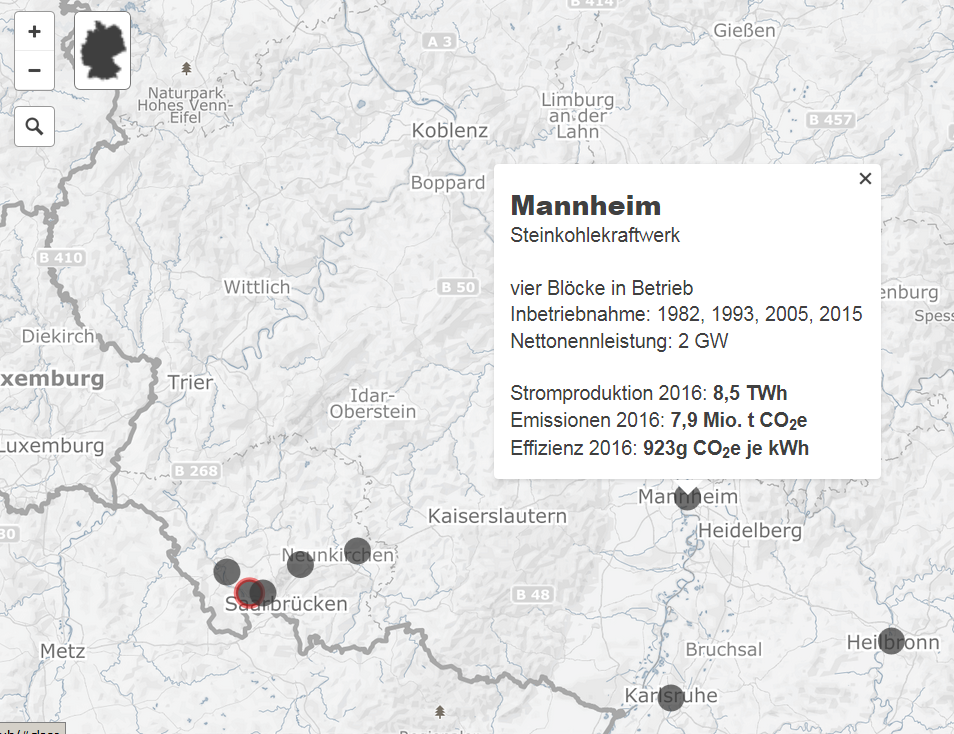
\includegraphics{figure/Kohle_mannheim.PNG}
\caption{}
\end{figure}

\end{block}

\end{frame}

\begin{frame}[fragile]{Das Paket \texttt{maps}}

\begin{Shaded}
\begin{Highlighting}[]
\KeywordTok{library}\NormalTok{(maps)}
\KeywordTok{data}\NormalTok{(world.cities)}
\KeywordTok{map}\NormalTok{(}\StringTok{"france"}\NormalTok{)}
\KeywordTok{map.cities}\NormalTok{(world.cities,}\DataTypeTok{col=}\StringTok{"blue"}\NormalTok{)}
\end{Highlighting}
\end{Shaded}

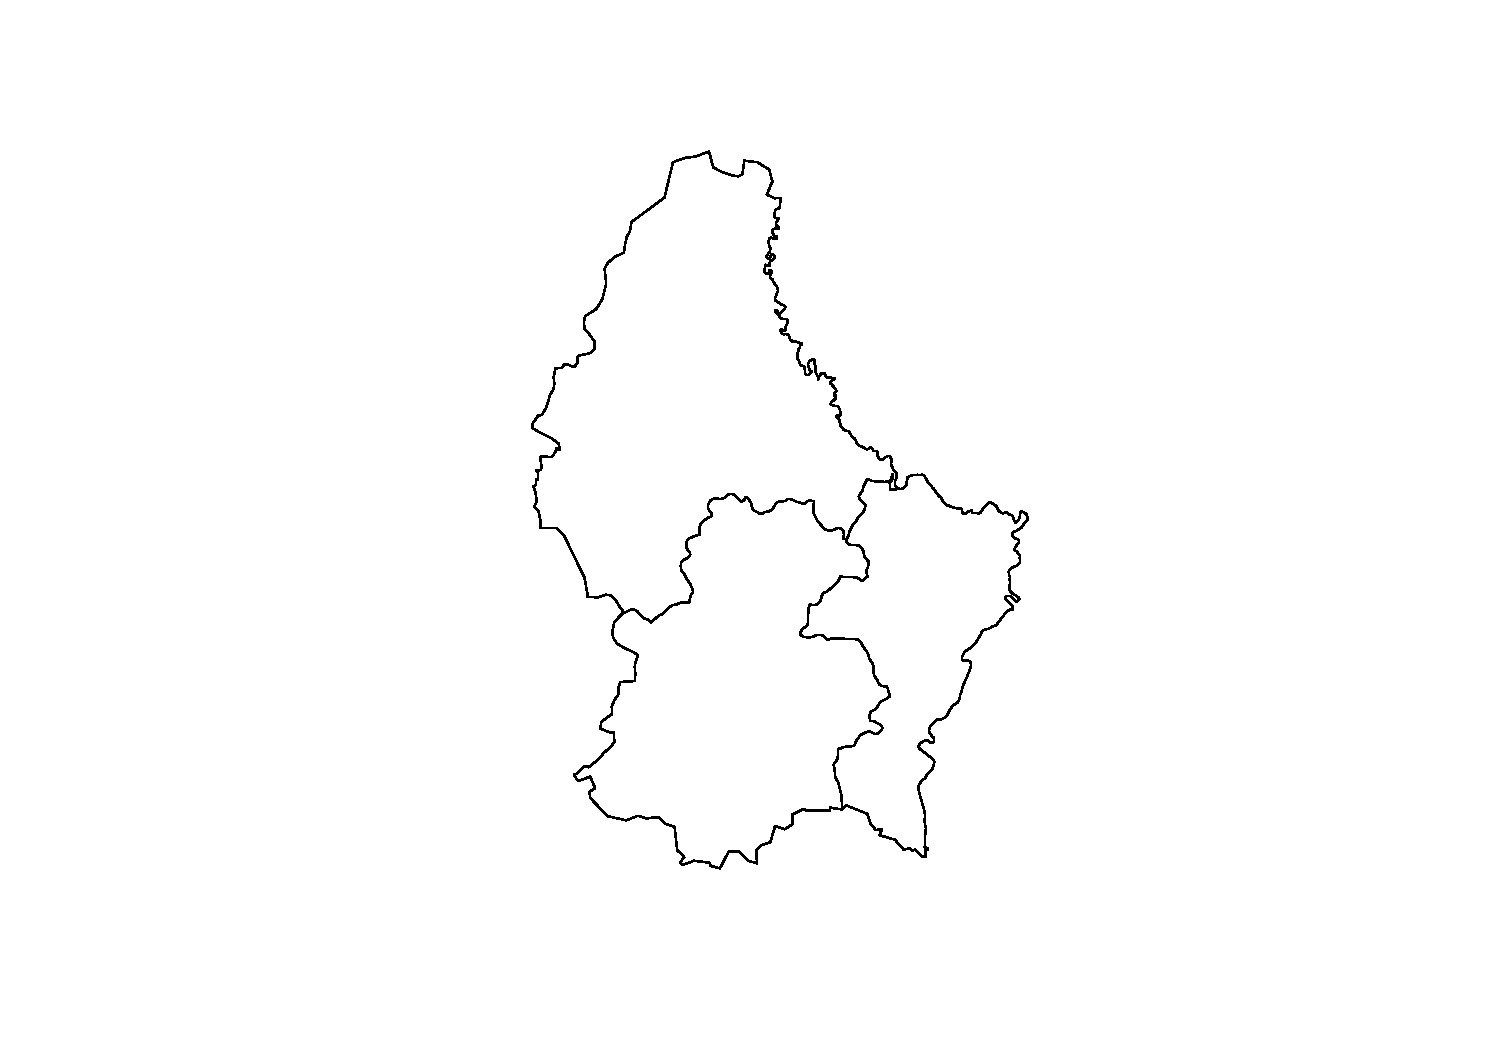
\includegraphics{ps_user_stuttgart_part3_files/figure-beamer/unnamed-chunk-5-1.pdf}

\end{frame}

\begin{frame}[fragile]{Grenzen sind recht grob}

\begin{Shaded}
\begin{Highlighting}[]
\KeywordTok{map}\NormalTok{(}\StringTok{"world"}\NormalTok{, }\StringTok{"Germany"}\NormalTok{)}
\end{Highlighting}
\end{Shaded}

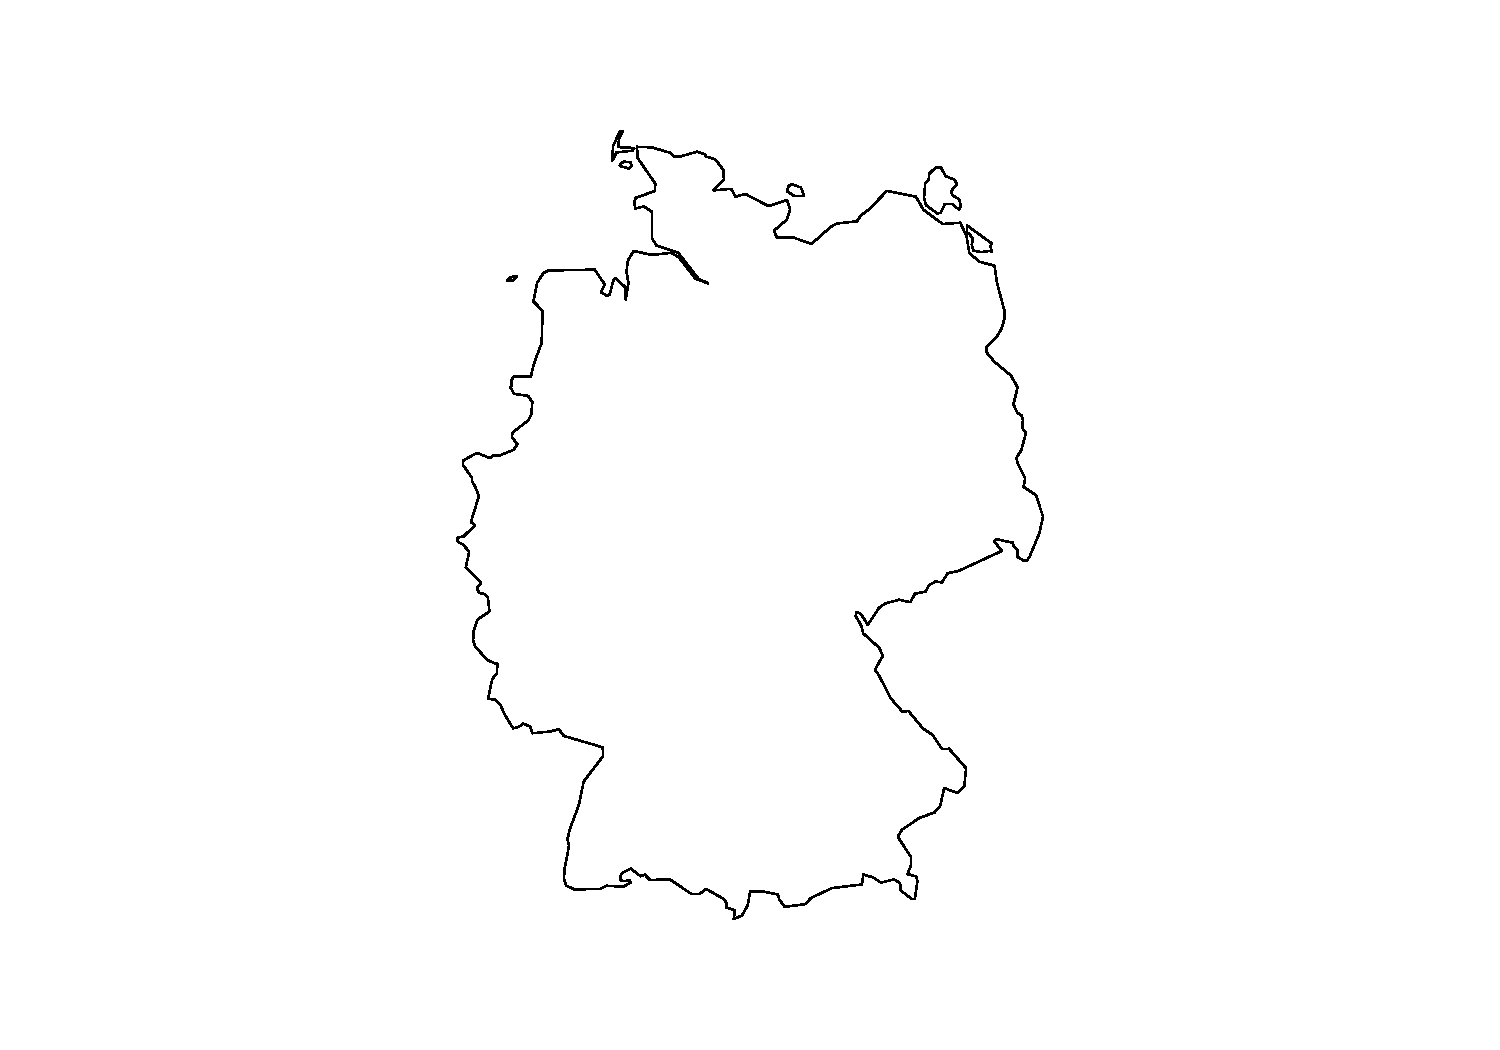
\includegraphics{ps_user_stuttgart_part3_files/figure-beamer/unnamed-chunk-6-1.pdf}

\end{frame}

\begin{frame}[fragile]{Das Paket \texttt{maptools}}

\begin{Shaded}
\begin{Highlighting}[]
\KeywordTok{library}\NormalTok{(maptools)}
\KeywordTok{data}\NormalTok{(wrld_simpl)}
\KeywordTok{plot}\NormalTok{(wrld_simpl,}\DataTypeTok{col=}\StringTok{"royalblue"}\NormalTok{)}
\end{Highlighting}
\end{Shaded}

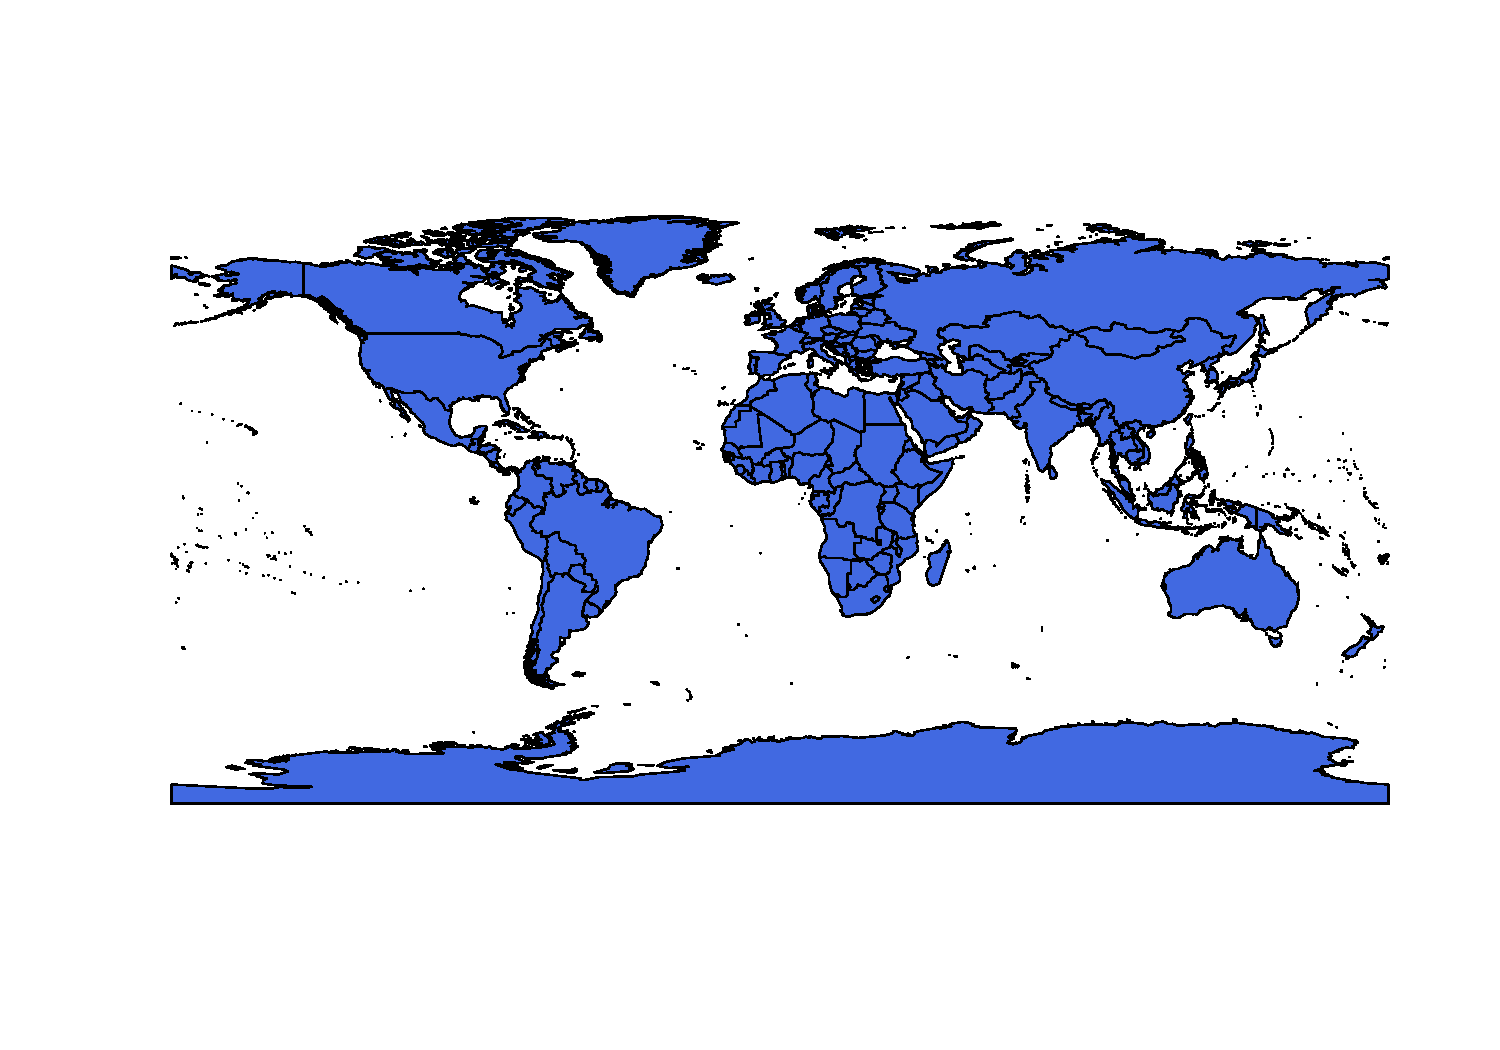
\includegraphics{ps_user_stuttgart_part3_files/figure-beamer/unnamed-chunk-7-1.pdf}

\end{frame}

\begin{frame}[fragile]{Das Paket \texttt{sp}}

\begin{Shaded}
\begin{Highlighting}[]
\KeywordTok{library}\NormalTok{(sp)}
\KeywordTok{spplot}\NormalTok{(wrld_simpl,}\StringTok{"POP2005"}\NormalTok{)}
\end{Highlighting}
\end{Shaded}

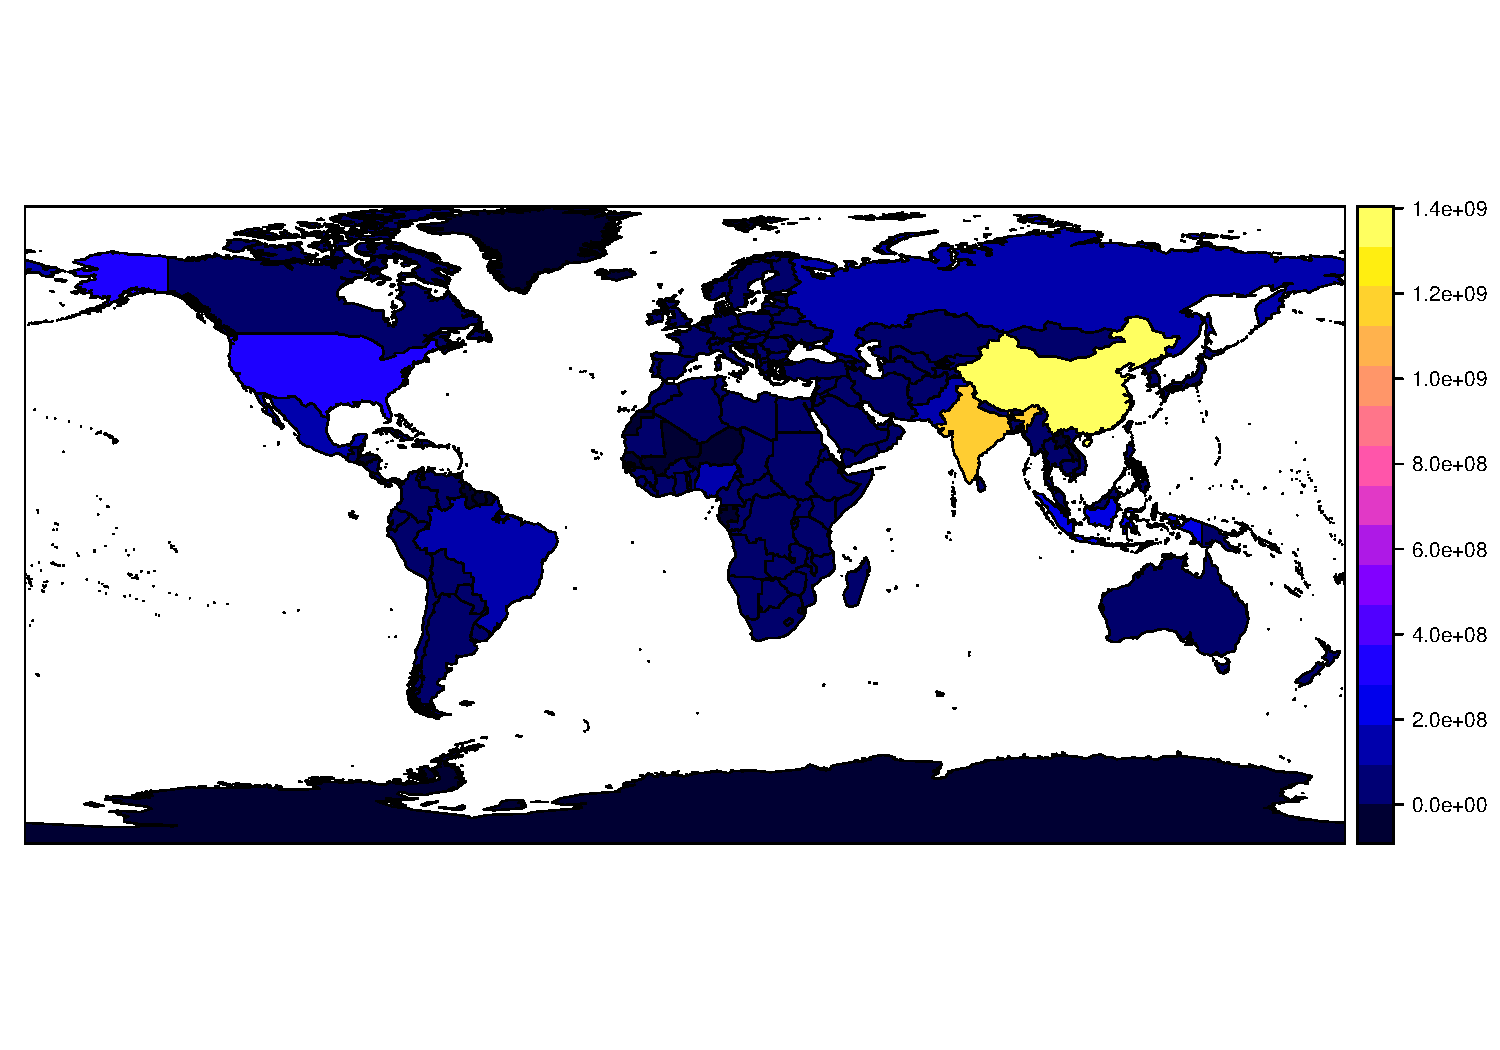
\includegraphics{ps_user_stuttgart_part3_files/figure-beamer/unnamed-chunk-8-1.pdf}

\end{frame}

\begin{frame}[fragile]{Das Paket \texttt{raster}}

\begin{Shaded}
\begin{Highlighting}[]
\KeywordTok{library}\NormalTok{(raster)}
\NormalTok{LUX1 <-}\StringTok{ }\KeywordTok{getData}\NormalTok{(}\StringTok{'GADM'}\NormalTok{, }\DataTypeTok{country=}\StringTok{'LUX'}\NormalTok{, }\DataTypeTok{level=}\DecValTok{1}\NormalTok{)}
\KeywordTok{plot}\NormalTok{(LUX1)}
\end{Highlighting}
\end{Shaded}

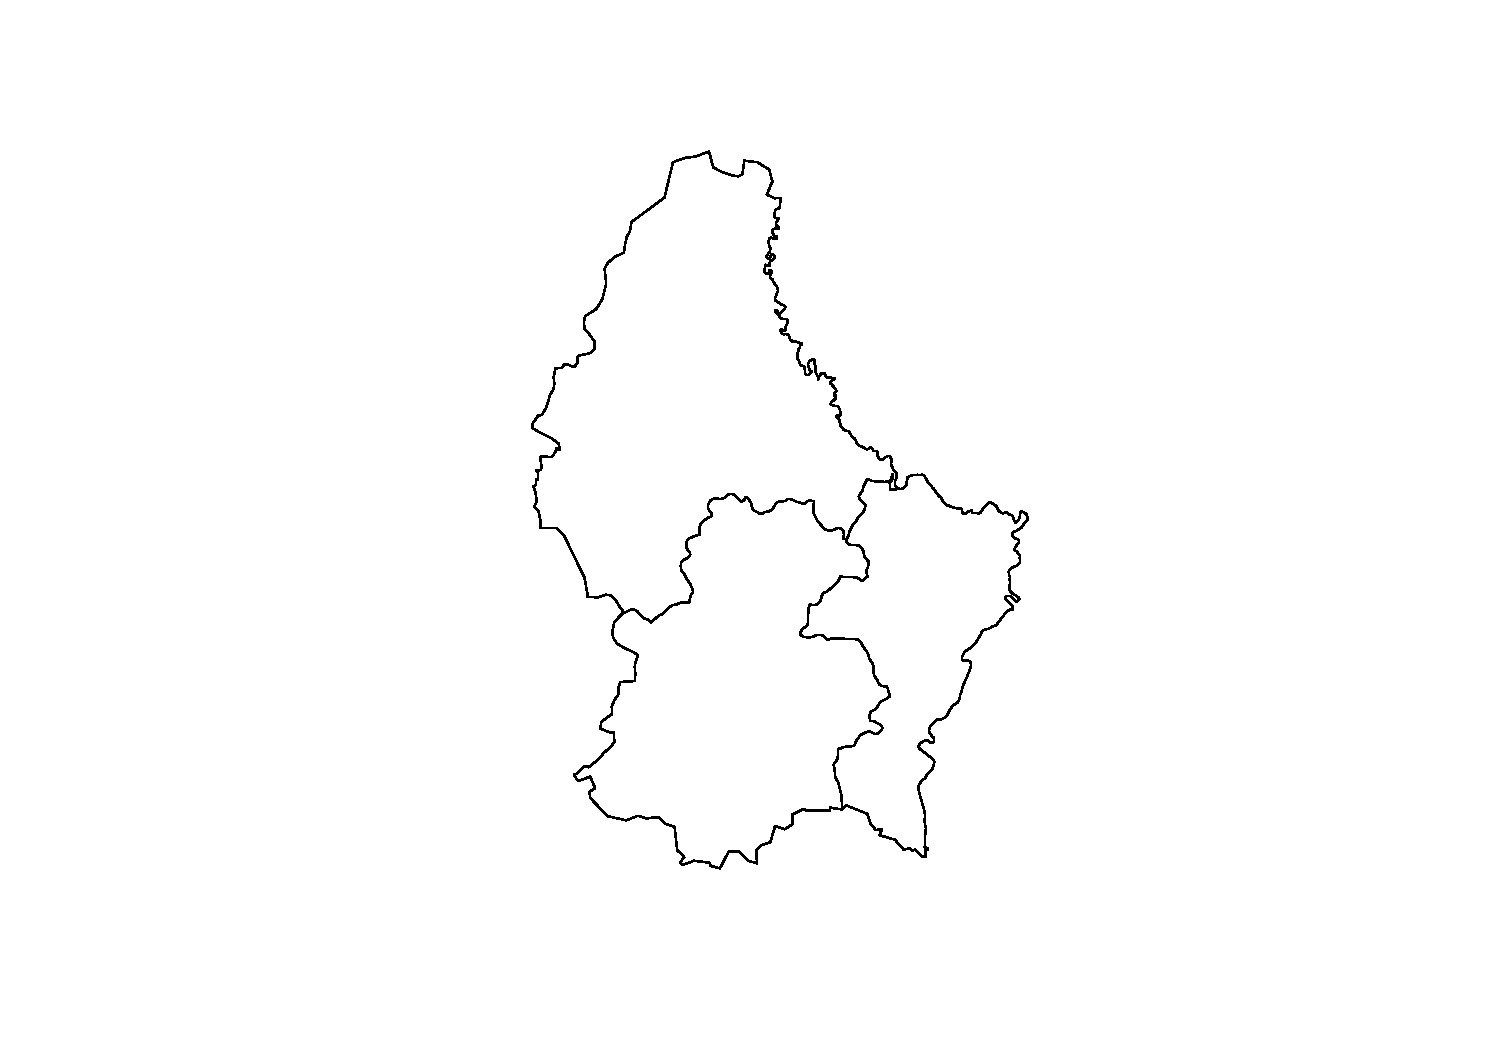
\includegraphics{ps_user_stuttgart_part3_files/figure-beamer/unnamed-chunk-9-1.pdf}

\end{frame}

\begin{frame}[fragile]{Daten für das Luxemburg Beispiel}

\begin{Shaded}
\begin{Highlighting}[]
\KeywordTok{kable}\NormalTok{(}\KeywordTok{head}\NormalTok{(LUX1}\OperatorTok{@}\NormalTok{data[,}\DecValTok{1}\OperatorTok{:}\DecValTok{6}\NormalTok{]))}
\end{Highlighting}
\end{Shaded}

\begin{longtable}[]{@{}rrllrl@{}}
\toprule
OBJECTID & ID\_0 & ISO & NAME\_0 & ID\_1 & NAME\_1\tabularnewline
\midrule
\endhead
1 & 131 & LUX & Luxembourg & 1 & Diekirch\tabularnewline
2 & 131 & LUX & Luxembourg & 2 & Grevenmacher\tabularnewline
3 & 131 & LUX & Luxembourg & 3 & Luxembourg\tabularnewline
\bottomrule
\end{longtable}

\end{frame}

\begin{frame}[fragile]{Kreise in Deutschland}

\begin{itemize}
\tightlist
\item
  Umrisse von 402 Kreisen in Deutschland
\item
  Quelle:
  \href{http://www.geodatenzentrum.de/geodaten/gdz_rahmen.gdz_div?gdz_spr=deu\&gdz_akt_zeile=5\&gdz_anz_zeile=1\&gdz_unt_zeile=15\&gdz_user_id=0}{Bundesamt
  für Kartographie und Geodäsie}
\item
  Karten gibt es auch für Bundesländer und Gemeinden
\end{itemize}

\begin{Shaded}
\begin{Highlighting}[]
\KeywordTok{library}\NormalTok{(maptools)}
\NormalTok{krs <-}\StringTok{ }\KeywordTok{readShapePoly}\NormalTok{(}\StringTok{"vg250_ebenen/vg250_krs.shp"}\NormalTok{)}
\KeywordTok{plot}\NormalTok{(krs)}
\end{Highlighting}
\end{Shaded}

\end{frame}

\begin{frame}[fragile]{Ortsnetzbereiche}

Quelle:
\href{https://www.bundesnetzagentur.de/DE/Sachgebiete/Telekommunikation/Unternehmen_Institutionen/Nummerierung/Rufnummern/ONRufnr/ON_Einteilung_ONB/ON_ONB_ONKz_ONBGrenzen_Basepage.html}{Bundesnetzagentur}

\begin{longtable}[]{@{}llll@{}}
\toprule
& VORWAHL & NAME & KENNUNG\tabularnewline
\midrule
\endhead
0 & 04651 & Sylt & NA\tabularnewline
1 & 04668 & Klanxbüll & NA\tabularnewline
2 & 04664 & Neukirchen b Niebüll & NA\tabularnewline
3 & 04663 & Süderlügum & NA\tabularnewline
4 & 04666 & Ladelund & NA\tabularnewline
5 & 04631 & Glücksburg Ostsee & NA\tabularnewline
\bottomrule
\end{longtable}

\begin{Shaded}
\begin{Highlighting}[]
\NormalTok{onb <-}\StringTok{ }\KeywordTok{readShapePoly}\NormalTok{(}\StringTok{"onb_grenzen.shp"}\NormalTok{)}
\KeywordTok{kable}\NormalTok{(}\KeywordTok{head}\NormalTok{(onb}\OperatorTok{@}\NormalTok{data))}
\end{Highlighting}
\end{Shaded}

\end{frame}

\begin{frame}[fragile]{Vorwahlbereiche in der Region Stuttgart}

\begin{Shaded}
\begin{Highlighting}[]
\NormalTok{vw_stg <-}\StringTok{ }\KeywordTok{c}\NormalTok{(}\StringTok{"0711"}\NormalTok{, }\StringTok{"07121"}\NormalTok{, }\StringTok{"07122"}\NormalTok{)}
\NormalTok{vw_reg_stg <-}\StringTok{ }\NormalTok{onb[onb}\OperatorTok{@}\NormalTok{data}\OperatorTok{$}\NormalTok{VORWAHL }\OperatorTok\StringTok{ }\NormalTok{vw_stg, ]}
\KeywordTok{plot}\NormalTok{(vw_reg_stg)}
\end{Highlighting}
\end{Shaded}

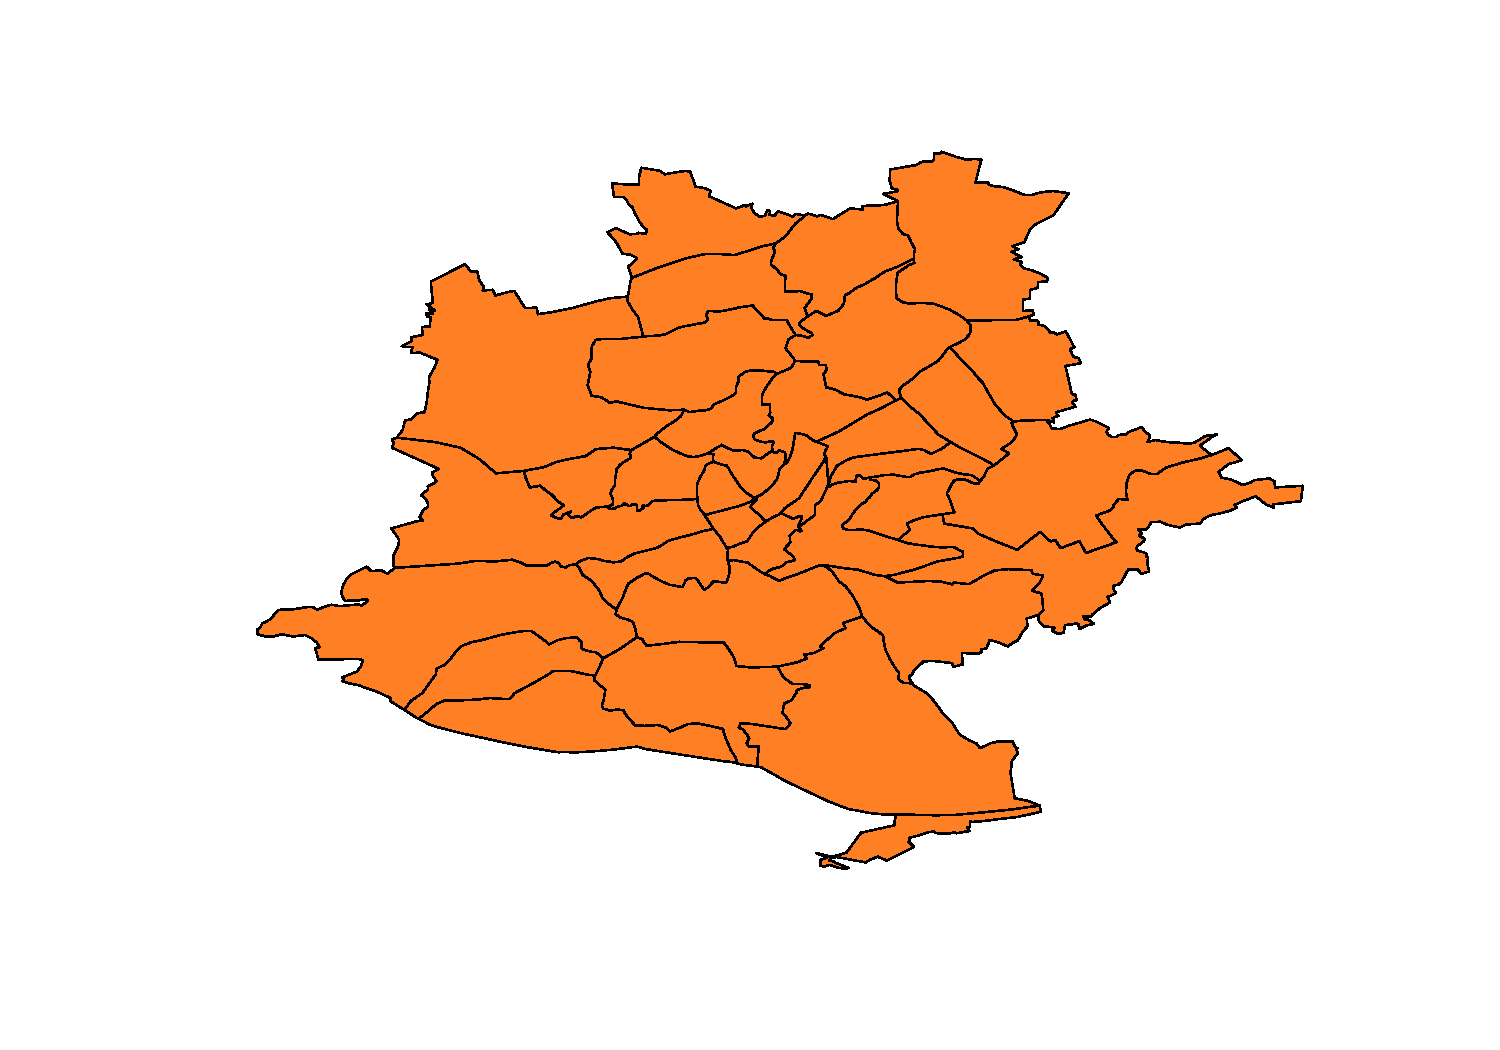
\includegraphics{ps_user_stuttgart_part3_files/figure-beamer/unnamed-chunk-16-1.pdf}

\begin{figure}
\centering
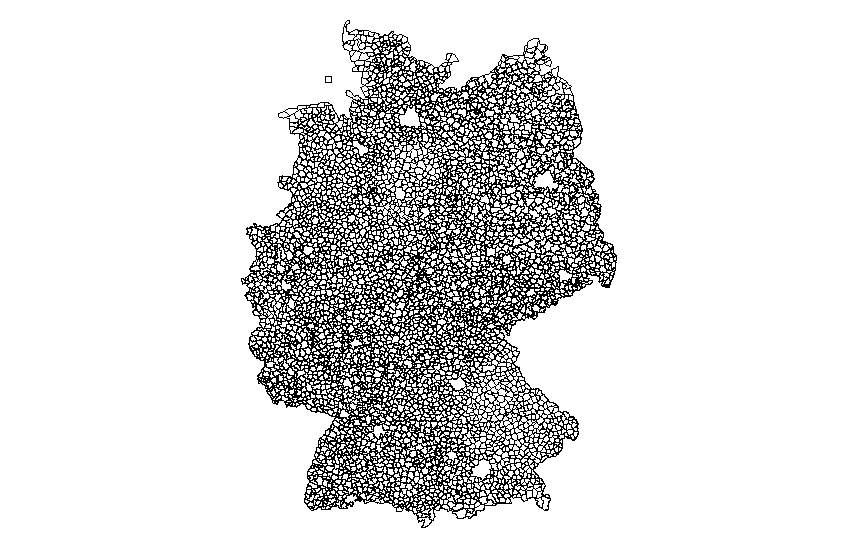
\includegraphics{https://raw.githubusercontent.com/Japhilko/GeoData/master/data/figure/onbGermany.png}
\caption{onbD}
\end{figure}

\end{frame}

\begin{frame}[fragile]{Einen größeren Vorwahlbereich ausschneiden}

\begin{Shaded}
\begin{Highlighting}[]
\NormalTok{vwb <-}\StringTok{ }\KeywordTok{as.character}\NormalTok{(onb}\OperatorTok{@}\NormalTok{data}\OperatorTok{$}\NormalTok{ONB_NUMMER)}
\NormalTok{vwb1 <-}\StringTok{ }\KeywordTok{substr}\NormalTok{(vwb, }\DecValTok{1}\NormalTok{,}\DecValTok{2}\NormalTok{)}
\NormalTok{vwb7 <-}\StringTok{ }\NormalTok{onb[vwb1}\OperatorTok{==}\StringTok{"07"}\NormalTok{,]}
\KeywordTok{plot}\NormalTok{(vwb7)}
\end{Highlighting}
\end{Shaded}


\includegraphics{ps_user_stuttgart_part3_files/figure-beamer/unnamed-chunk-17-1.pdf}

\end{frame}

\begin{frame}[fragile]{Das Paket \texttt{rgdal}}

\begin{itemize}
\tightlist
\item
  Postleitzahlenbereiche - \url{http://arnulf.us/PLZ}
\end{itemize}

\begin{Shaded}
\begin{Highlighting}[]
\KeywordTok{library}\NormalTok{(rgdal)}
\end{Highlighting}
\end{Shaded}

\begin{verbatim}
## OGR data source with driver: ESRI Shapefile 
## Source: "post_pl.shp", layer: "post_pl"
## with 8270 features
## It has 3 fields
\end{verbatim}

\begin{Shaded}
\begin{Highlighting}[]
\KeywordTok{setwd}\NormalTok{(}\StringTok{"D:/GESIS/Workshops/GeoDaten/data/"}\NormalTok{)}
\NormalTok{PLZ <-}\StringTok{ }\KeywordTok{readOGR}\NormalTok{ (}\StringTok{"post_pl.shp"}\NormalTok{,}\StringTok{"post_pl"}\NormalTok{)}
\end{Highlighting}
\end{Shaded}

\begin{Shaded}
\begin{Highlighting}[]
\KeywordTok{library}\NormalTok{(rgdal)}
\NormalTok{PLZ <-}\StringTok{ }\KeywordTok{readOGR}\NormalTok{ (}\StringTok{"post_pl.shp"}\NormalTok{,}\StringTok{"post_pl"}\NormalTok{)}
\end{Highlighting}
\end{Shaded}

\end{frame}

\begin{frame}[fragile]{PLZ-Bereiche in Stuttgart}

\begin{Shaded}
\begin{Highlighting}[]
\NormalTok{SG <-}\StringTok{ }\NormalTok{PLZ[PLZ}\OperatorTok{@}\NormalTok{data}\OperatorTok{$}\NormalTok{PLZORT99}\OperatorTok{==}\StringTok{"Stuttgart"}\NormalTok{,]}
\KeywordTok{plot}\NormalTok{(SG,}\DataTypeTok{col=}\StringTok{"chocolate1"}\NormalTok{)}
\end{Highlighting}
\end{Shaded}

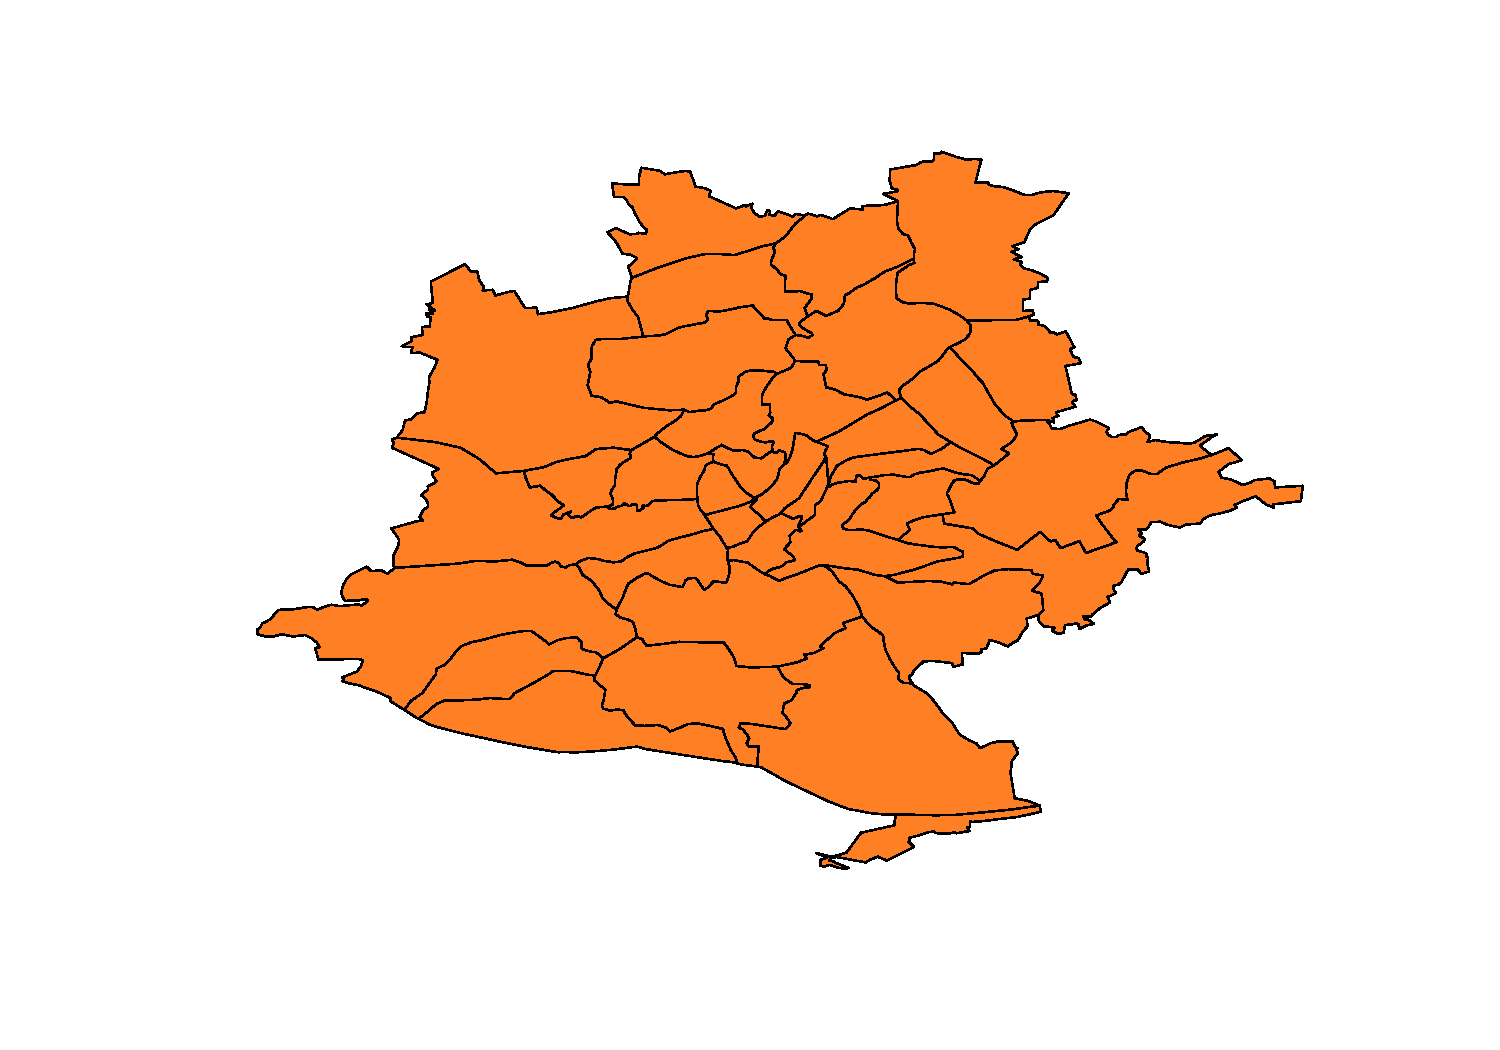
\includegraphics{ps_user_stuttgart_part3_files/figure-beamer/unnamed-chunk-22-1.pdf}

\end{frame}

\begin{frame}[fragile]{PLZ-Bereiche in Berlin}

\begin{Shaded}
\begin{Highlighting}[]
\NormalTok{BE <-}\StringTok{ }\NormalTok{PLZ[PLZ}\OperatorTok{@}\NormalTok{data}\OperatorTok{$}\NormalTok{PLZORT99}\OperatorTok\KeywordTok{c}\NormalTok{(}\StringTok{"Berlin-West"}\NormalTok{,}\StringTok{"Berlin (östl. Stadtbezirke)"}\NormalTok{),]}
\KeywordTok{plot}\NormalTok{(BE,}\DataTypeTok{col=}\StringTok{"chocolate2"}\NormalTok{)}
\end{Highlighting}
\end{Shaded}

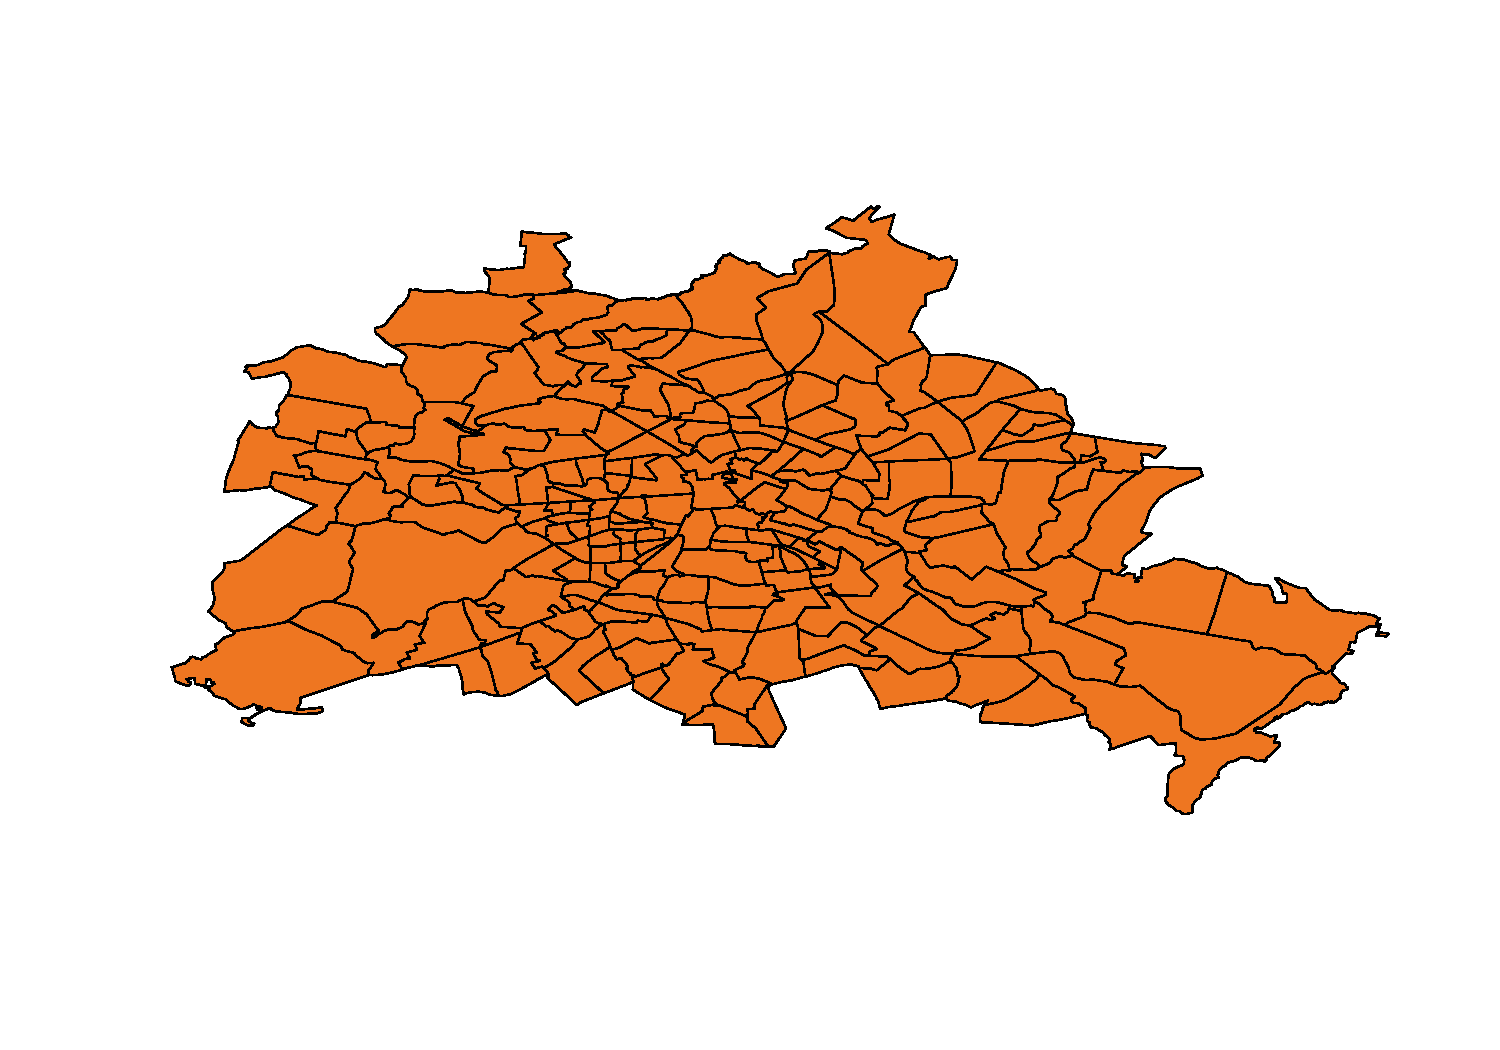
\includegraphics{ps_user_stuttgart_part3_files/figure-beamer/unnamed-chunk-23-1.pdf}

\end{frame}

\begin{frame}{Exkurs - Open Street Map}

\textless{}www.openstreetmap.org/export\textgreater{}

\begin{figure}
\centering
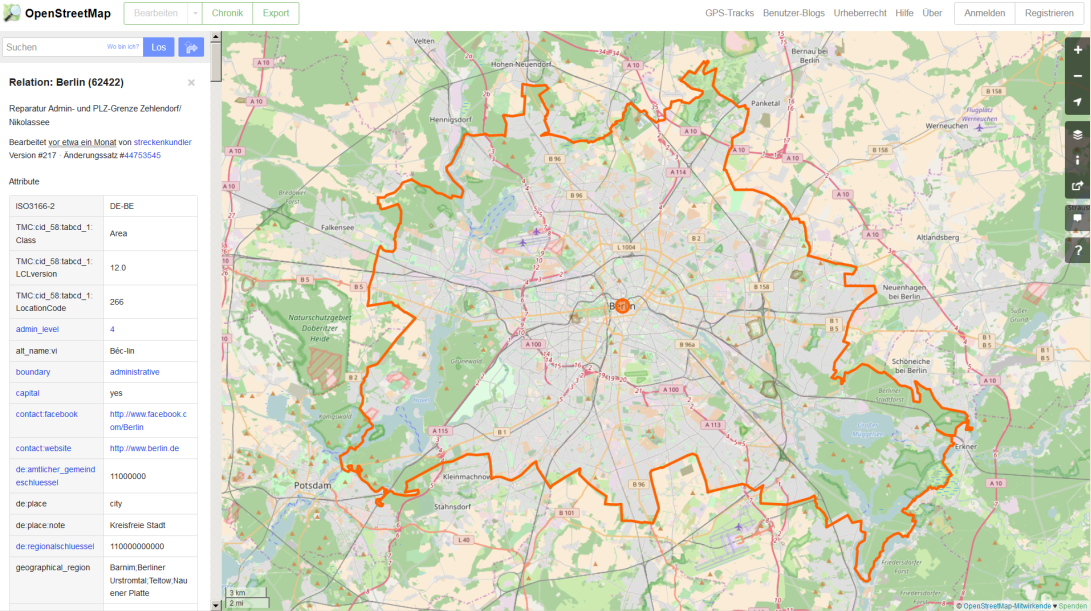
\includegraphics{https://github.com/Japhilko/GeoData/blob/master/2017/slides/figure/admgrBer.PNG}
\caption{}
\end{figure}

\end{frame}

\begin{frame}{\href{http://wiki.openstreetmap.org/wiki/Map_Features}{OpenStreetMap
- Map Features}}

\begin{figure}
\centering
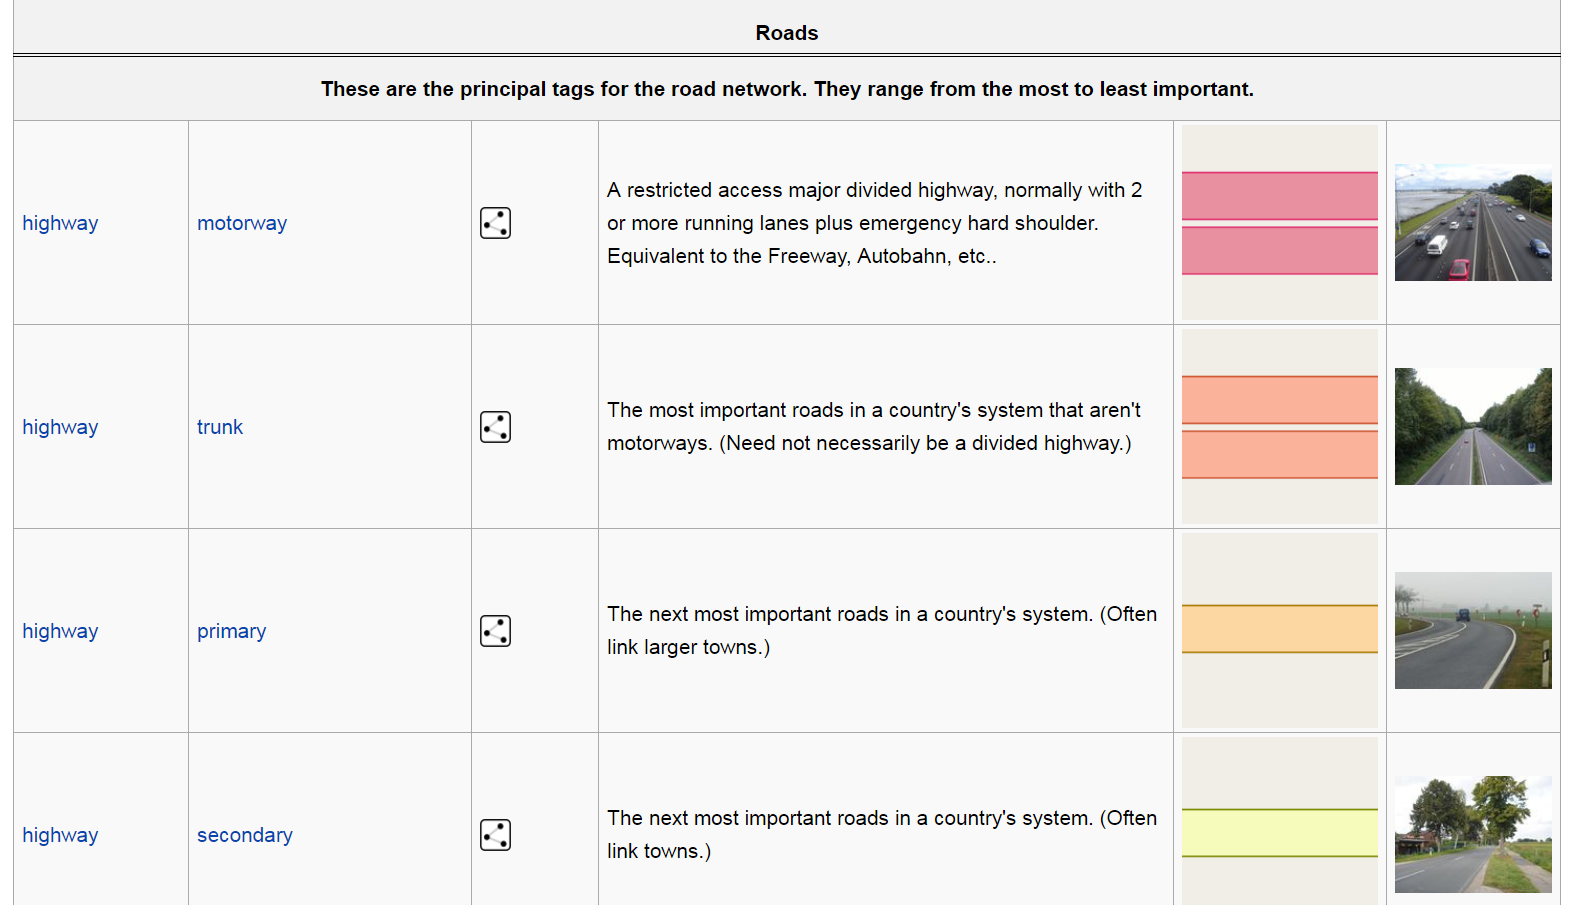
\includegraphics{figure/OSMroads.PNG}
\caption{}
\end{figure}

\end{frame}

\begin{frame}[fragile]{Daten verbinden - Bäckereien in Berlin}

\begin{Shaded}
\begin{Highlighting}[]
\NormalTok{(}\KeywordTok{load}\NormalTok{(}\StringTok{"data/info_bar_Berlin.RData"}\NormalTok{))}
\end{Highlighting}
\end{Shaded}

\end{frame}

\begin{frame}[fragile]{Matching}

\begin{Shaded}
\begin{Highlighting}[]
\NormalTok{tab_plz <-}\StringTok{ }\KeywordTok{table}\NormalTok{(info_be}\OperatorTok{$}\NormalTok{addr.postcode)}
\end{Highlighting}
\end{Shaded}

\begin{Shaded}
\begin{Highlighting}[]
\NormalTok{ind <-}\StringTok{ }\KeywordTok{match}\NormalTok{(BE}\OperatorTok{@}\NormalTok{data}\OperatorTok{$}\NormalTok{PLZ99_N,}\KeywordTok{names}\NormalTok{(tab_plz))}
\NormalTok{ind}
\end{Highlighting}
\end{Shaded}

\end{frame}

\begin{frame}[fragile]{Daten anspielen}

\begin{Shaded}
\begin{Highlighting}[]
\NormalTok{BE}\OperatorTok{@}\NormalTok{data}\OperatorTok{$}\NormalTok{num_plz <-}\StringTok{ }\NormalTok{tab_plz[ind]}
\end{Highlighting}
\end{Shaded}

\end{frame}

\begin{frame}[fragile]{Das Paket \texttt{tmap}}

\begin{Shaded}
\begin{Highlighting}[]
\KeywordTok{library}\NormalTok{(tmap)}
\end{Highlighting}
\end{Shaded}

\begin{Shaded}
\begin{Highlighting}[]
\NormalTok{BE}\OperatorTok{@}\NormalTok{data}\OperatorTok{$}\NormalTok{num_plz[}\KeywordTok{is.na}\NormalTok{(BE}\OperatorTok{@}\NormalTok{data}\OperatorTok{$}\NormalTok{num_plz)] <-}\StringTok{ }\DecValTok{0}
\KeywordTok{qtm}\NormalTok{(BE,}\DataTypeTok{fill =} \StringTok{"num_plz"}\NormalTok{)}
\end{Highlighting}
\end{Shaded}

\end{frame}

\begin{frame}{Zensus Atlas}

\url{https://ergebnisse.zensus2011.de/}

\begin{figure}
\centering
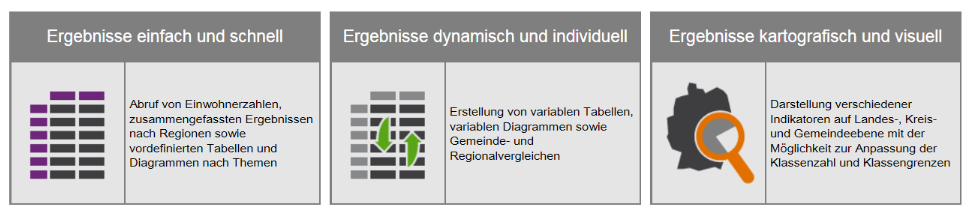
\includegraphics{https://raw.githubusercontent.com/Japhilko/GeoData/master/2017/slides/figure/Zensusdtb.PNG}
\caption{Zensus Datenbank}
\end{figure}

\end{frame}
